\documentclass[thesis.tex]{subfiles}
\begin{document}

\chapter{Main}\label{chap:basics}

\section{Overview}
Inspired by Lensing's LightSkin approach~\cite{bib:LightskinPaper}, we want to compute indirect lighting only at specific locations and interpolate the results over multiple pixels, as opposed to techniques like Reflective Shadow Maps or Voxel Cone Tracing \todo{ref related work sections}.
\todo{Advantages/disadvantages}
As in many previous works, we call these locations \emph{Light Caches}.

Our technique consists of three basic steps which are executed in every frame: Cache allocation, indirect lighting and cache interpolation.
The cache allocation pass assigns cells on a regular grid to cache memory, thus creating the caches that are about to be used in this frame.
Using a reflective shadow map, indirect lighting is then computed for all caches.
Finally each pixel interpolates an indirect lighting value using all neighboring caches within the grid.

Each of the following major sections will explain one of these stages and their interdependencies.
The last major section of this chapter will elaborate several implementation details, some of them crucial to the overall performance.\\
Many parts of our approach are based on several well-known techniques of which most have already been discussed in \autoref{chap:prevwork} and \autoref{chap:basics}.
Where necessary, details of the respective algorithms will be elaborated to address specifics implied by the overall technique.

\section{Cache Allocation}
Since the goal of this work is a fully dynamic solution that works without any pre-computations, it is necessary to place all caches at runtime, as opposed to LightSkin~\cite{bib:LightskinPaper} where caches are placed in a computational intense preprocessing step.
Before we introduce our solution, several general implications of such an approach are elaborated.

\subsection{General Properties and Requirements of Dynamic Cache Placement}
Compared to a precomputation based approach, there are several intrinsic advantages which can be expected of a dynamic light cache placement.
Since we target for a single bounce of indirect light, caches are only used by locations that lie in the current view frustum (for multiple bounces however, it might be necessary to transfer lights between caches).
Also it should be possible to decrease the number of caches for distant objects, thus keeping screen-space cache density within a given bound.
Both properties result in a much lower memory footprint especially for large scenes.

While it can be very beneficial to place caches dependent on the current view, this also may introduce several temporal artifacts if caches disappear or move, i.e. strong changes in indirect lighting from one frame to the next.
Additionally, it is necessary to guarantee that target pixels have easy access to a certain number of caches to be able to interpolate them.
Note that the interpolation pass can have temporal coherence problems on its own, as the assignment of a cache to its surrounding world positions needs to be stable, no matter how densely they are sampled, i.e. how many pixels a given world space area covers.

So far, the data requirements of each cache have not been defined yet.
Precomputed caches can naturally hold almost arbitrary data (as long as a given memory bound is not exceeded).
Dynamic caches on the other hand need to acquire their data every frame, which is not only costly performance-wise but may also cancel out certain types of data as it may not be accessible. For example LightSkin~\cite{bib:LightskinPaper} needs to a rather complex area metric for each cache that can not be computed in real-time.
Naturally, such constraints also affect the following lighting and interpolation stages tremendously.

We evaluated several approaches before we came up with our final algorithm.
If you are interested you can read the summary of these attempts in \autoref{chap:abandoned}.

\subsection{Adaptive Real-Time (Ir-)Radiance Volumes} \todo{Better name?}
To cancel out temporal artifacts entirely, we decided to place caches only on the nodes of a regular grid in world space.
The main disadvantage of this method is, that cache are not placed on surfaces and thus have no concrete orientation.

During the cache allocation pass, each pixel activates its eight nearest caches.
This is done by screen pass, using the depth buffer from the previously rendered scene.
\todo{write: allows for optimizations since neighboring pixels activate the same cache - see blabla}

The grid moves with the view frustum to cover it entirely.
However, all movements are snapped to the distance between two caches, since smooth movements would lead again to temporal incoherences.

Even so, usually only a very small fraction of all grid cells contains an activated cache.
use grid for addresses only
large buffer with all cache data instead,
what does a cache contain?

\subsection{Cascading}

\section{Indirect Lighting}

need rsm ... 


Different basis: SH1, SH2, H4, H6
It is possible to use hemispherical basis to represent the irradiance for a given normal, since for a given view, the possible normal directions are limited to a hemisphere. ....

\subsection{Indirect Shadows}

\subsubsection{Scene Voxelization}

\subsubsection{Cone Casts on Filtered Reflective Shadow Maps}


\section{Cache Interpolation}



\section{Implementation}

\emph{As many as possible details should be delayed into this chapter. If it gets large or starts to mirror the main part, make it a chapter!}

This is the right place for describing how to use Compute, OpenGL etc. for achieving the rather abstract formulated goals of the sections before.

Deferred Renderer, 32bits per Layer RGB(A) srgb - Diffuse, RG 16snorm - Normals with angles, extra infos todo, R32F Depth Buffer (swapped near/far)\\
(This detail belongs more or less to Eva...)

\subsection{Pipeline Overview}

\begin{figure}[h]
	\centering
	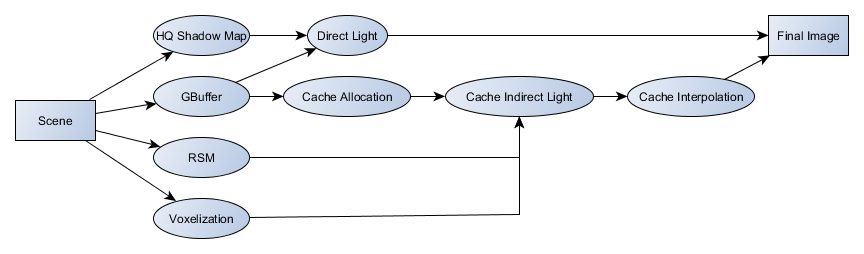
\includegraphics[width=\textwidth]{renderingpipeline_draft}
\end{figure}

\todo{same with image}

\todo{explanation}

\subsection{Cache Allocation}
cacheList via shared memory etc.
"Adress Coord Cache"

\subfilebib % Makes bibliography available when compiling as subfile
\end{document}